\documentclass[a4paper,ngerman]{scrartcl}
\renewcommand{\rmdefault}{cmr}
\renewcommand{\sfdefault}{cmss}
\renewcommand{\ttdefault}{cmtt}
\usepackage[T1]{fontenc}
\usepackage[utf8]{inputenc}
\usepackage{array}
\usepackage{refstyle}
\usepackage{float}
\usepackage{enumitem}
\usepackage{amsmath}
%\usepackage{euler}
\usepackage{hyperref}
\makeatletter
\usepackage{multirow}
\usepackage{isotope}
\usepackage{tikz-uml}
\usepackage[section]{placeins}
\flushbottom
\usepackage{geometry}
\geometry{a4paper}
\usepackage[headsepline]{scrpage2}
\usepackage{color}
\usetikzlibrary{circuits.ee.IEC}
%\usepackage{beramono}
\usepackage{pdfpages}
\makeatother
%\usepackage{babel}
\usepackage{listings}
\lstset{language=verilog,
basicstyle={\footnotesize\fontfamily{fvm}\selectfont},
commentstyle={\textit},
keywordstyle={\bfseries},
tabsize=4,
frame=leftline,
numbers=left,
numberstyle={\tiny}}
\usepackage{siunitx}
\title{MIX-fpga}
\author{Michael Schröder \\ \href{mi.schroeder@netcologne.de}{mi.schroeder@netcologne.de}}
\usepackage[
type={CC},
modifier={by-nc-sa},
version={3.0},
]{doclicense}
\begin{document}

\maketitle

\section{A real MIX}

Have you ever heard of Don Knuths (hypothetical) first polyunsaturated computer MIX, the 1009? In this project we will build a binary version of the MIX-Computer as described in "The Art of Computer Programming, Vol. 1" by Donald E. Knuth running on an fpga-board.

The presented implementation is based on the fpga development board iCE40HX8K-EVB from the company Olimex Ltd.\footnote{\href{www.olimex.com}{www.olimex.com}}, which has the nice property of being completely open source. The whole project uses only FOSS free and open source hard- and software, so everybody can build their own MIX following the instructions on the project site\footnote{\href{www.gitlab.com/x653/mix-fpga}{www.gitlab.com/x653/mix-fpga}}.

\begin{figure}[H]
	\centering
	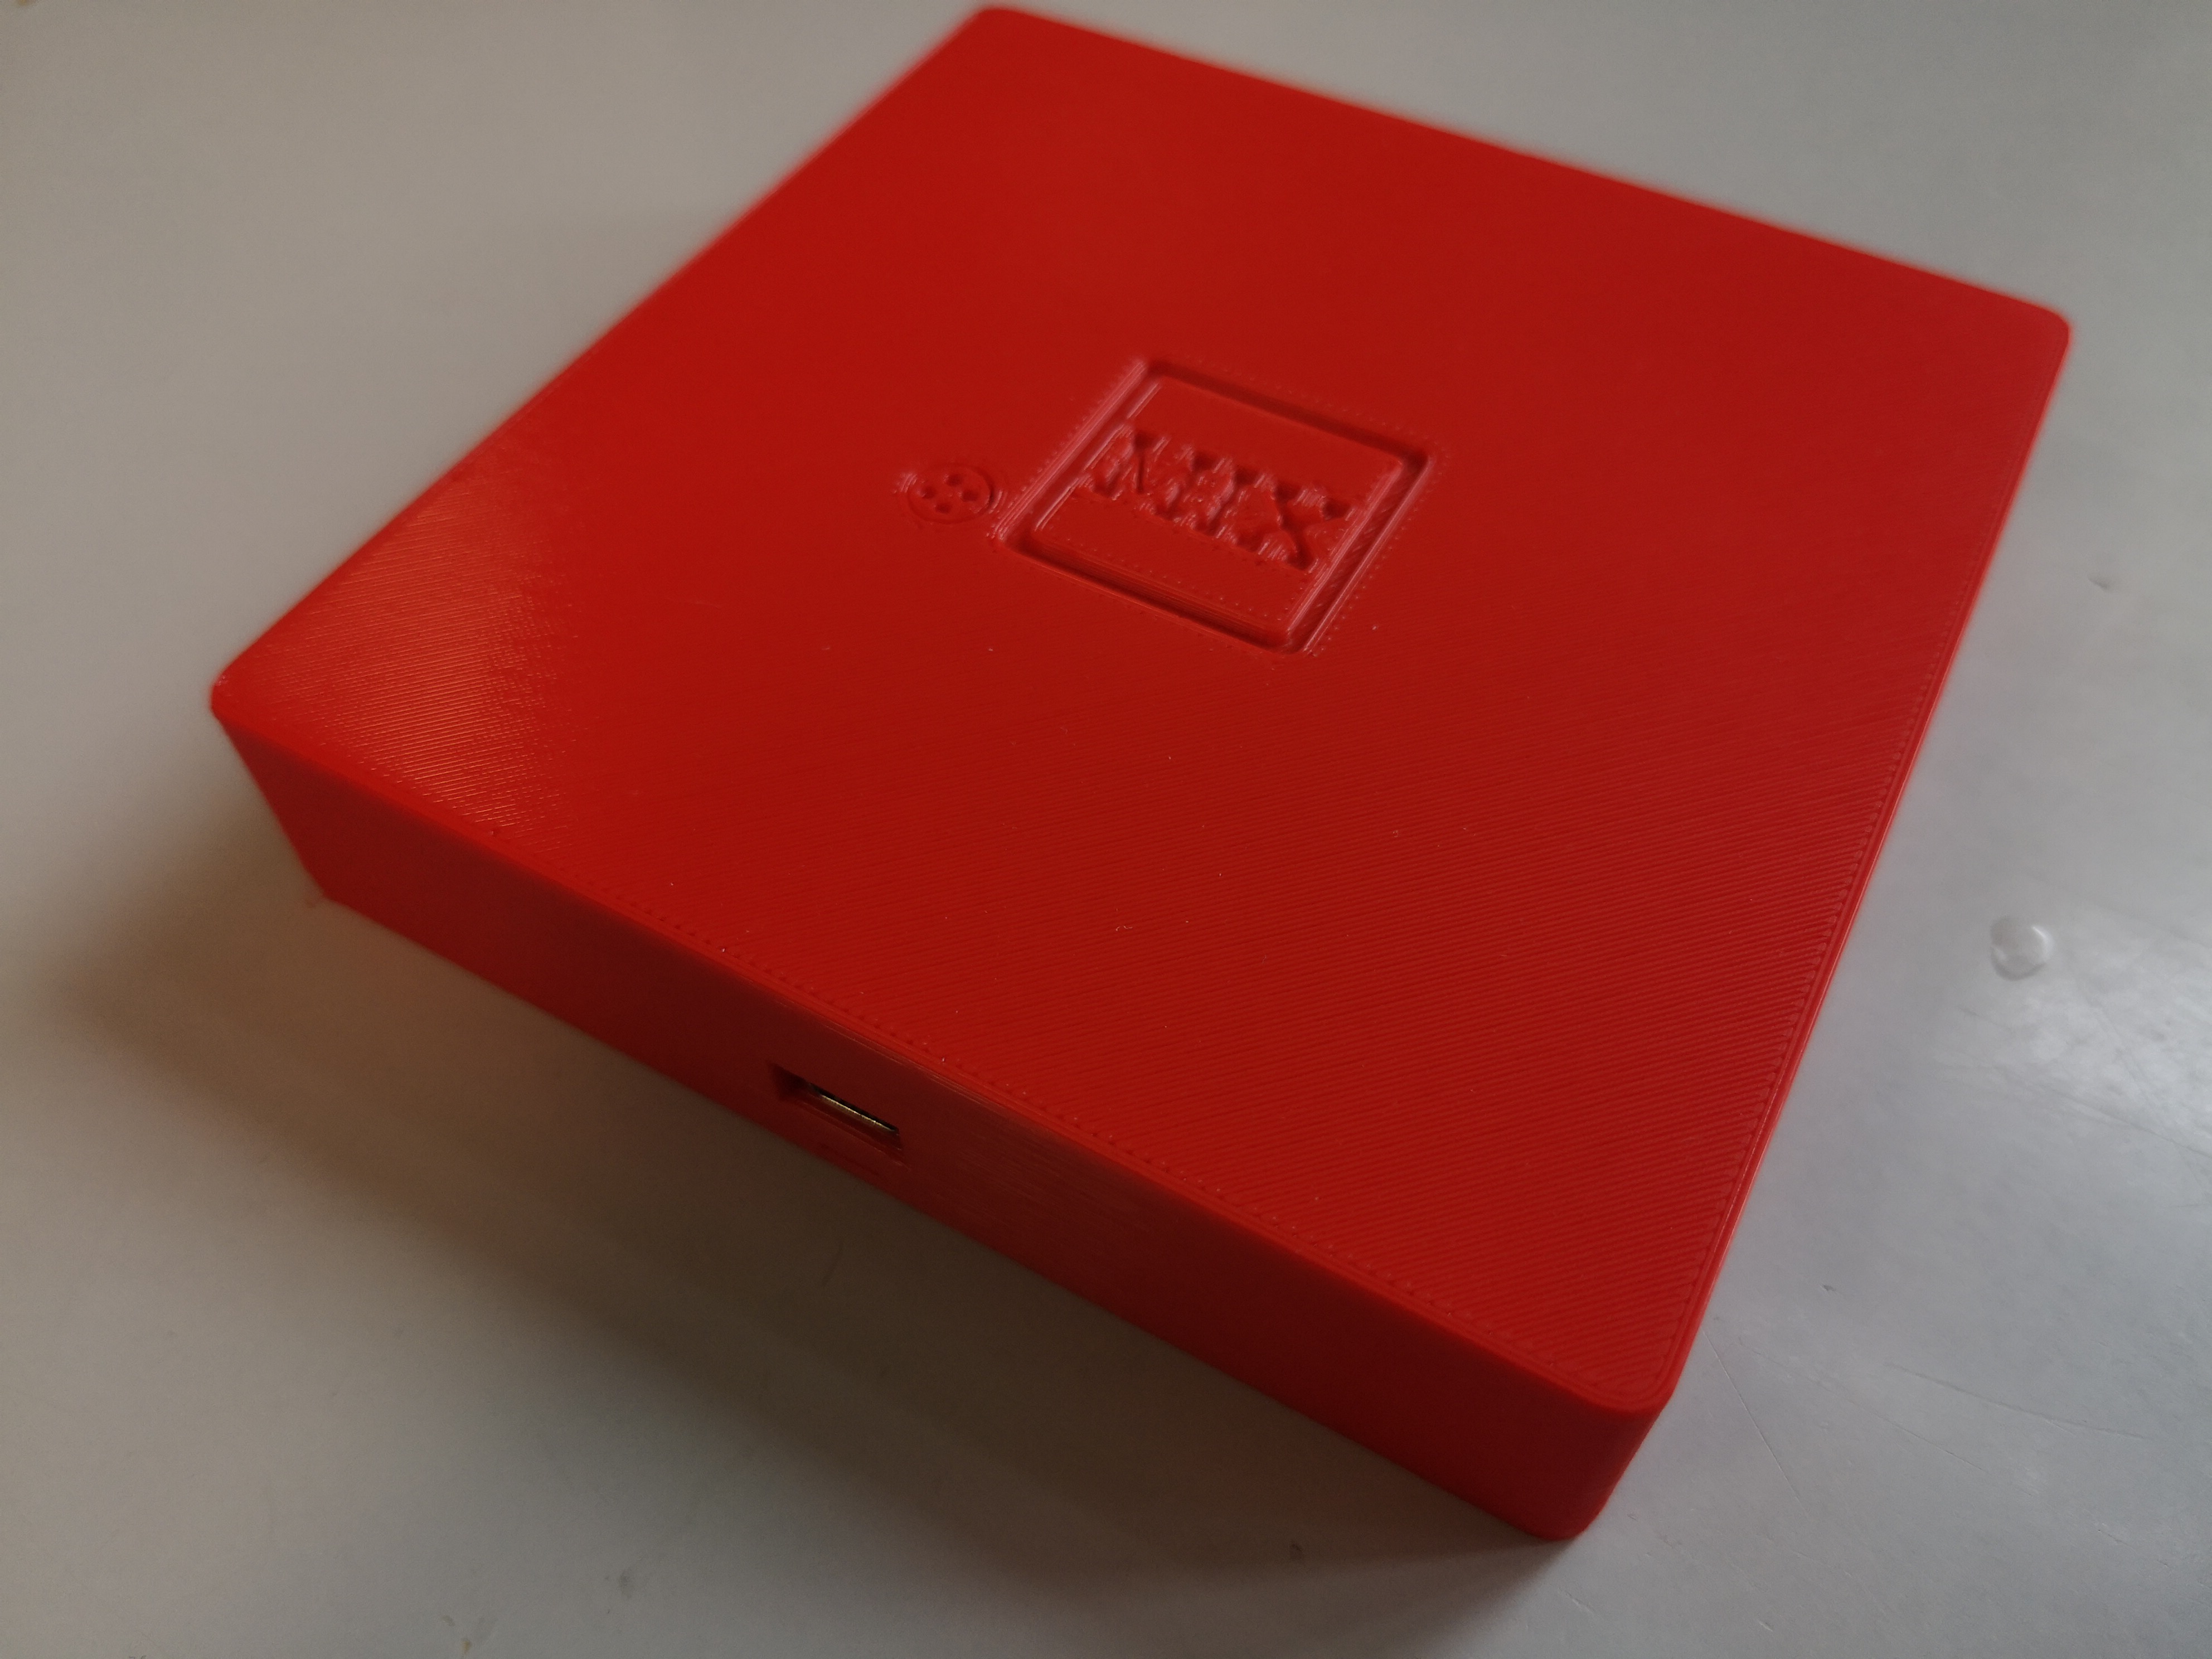
\includegraphics[width=0.6\linewidth]{../MIX_real.jpg}
	\caption{The real MIX}
	\label{fig:mixtoast}
\end{figure}

\subsection{A look inside}

The MIX computer is composed of two little boards.

\begin{enumerate}
	\item iCE40HX8K-EVB\footnote{\href{www.olimex.com/Products/FPGA/iCE40/iCE40HX8K-EVB}{www.olimex.com/Products/FPGA/iCE40/iCE40HX8K-EVB}}, the fpga development board from the company Olimex Ltd.	
	\item  USB-serial adapter\footnote{\href{www.olimex.com/Products/Breadboarding/BB-CH340T}{www.olimex.com/Products/Breadboarding/BB-CH340T}}. Used to power the board with 5V and to in-/output data over the serial interface.
\end{enumerate}

\begin{figure}[H]
	\centering
	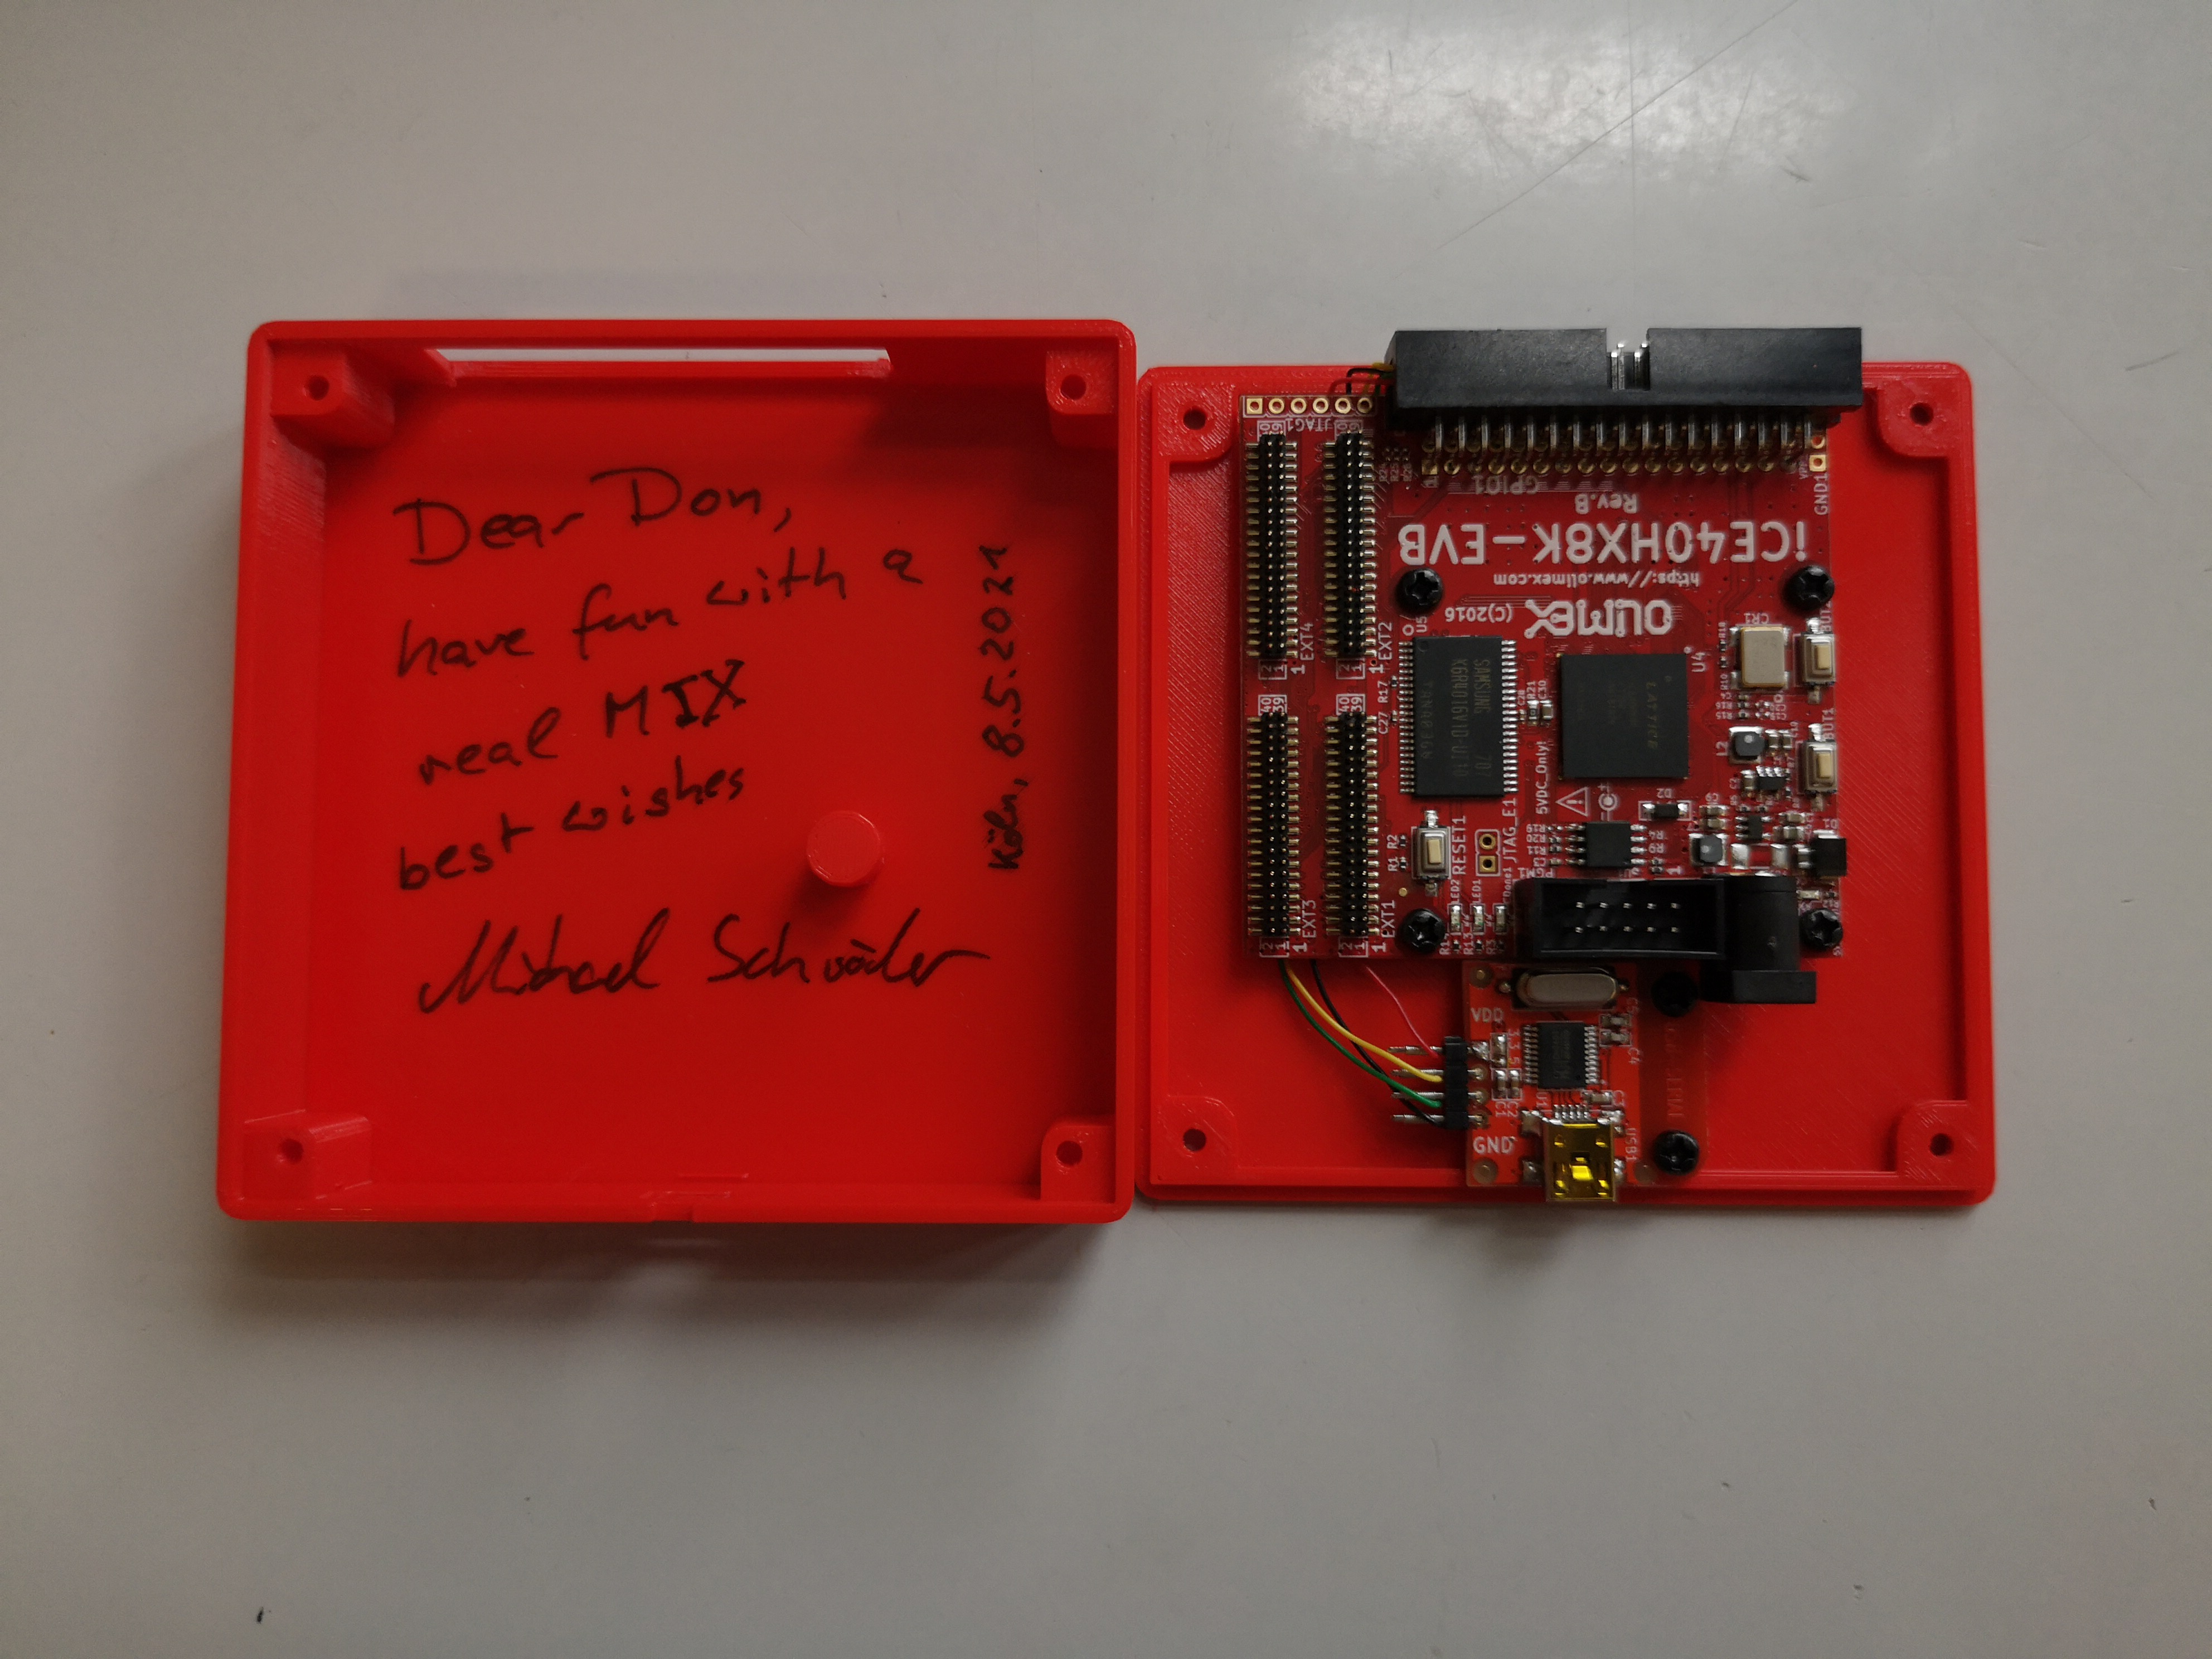
\includegraphics[width=0.7\linewidth]{../MIX_don.jpg}
	\caption{Look inside and see the two boards interconnected with wire wrap technique}
	\label{fig:mixinside}
\end{figure}


\subsection{Specifications}

\subsubsection{clock}
MIX runs on iCE40HX8K-EVB clocked at \SI{25}{MHz}. The fundamental unit of time $u$ corresponds to $1u = \SI{40}{ns}$, so according to Knuth it's a relatively high priced machine.

\subsubsection{character based I/O units}
In our MIX implementation all character based I/O units (U16 -- U20) are connected to the USB-connector and can be accessed as serial data streams. You can connect MIX with any PC running a terminal emulator (e.g. screen for linux). The terminal should be set to 115200 baud (8N1). A conversion between ASCII and Knuths character codes is done in hardware according to Knuths specification (see TAOCP p. 128).

\subsubsection{The block based I/O unit U8}
A block based device is implemented on I/O unit 8. The device acts as a disk with 1000 blocks à 100 words. The data is stored in the SRAM chip found on the iCE40HX8K-EVB board. The speed of read and write operations is exactly 401 $u$ for reading or writing one complete block of data (no JBUS is needed). The data stored to unit U8 can be retrieved also after a reset (Go-Button). But on a full shutdown, when removing power supply (USB connector) data is lost.

\begin{figure}[H]
	\centering
	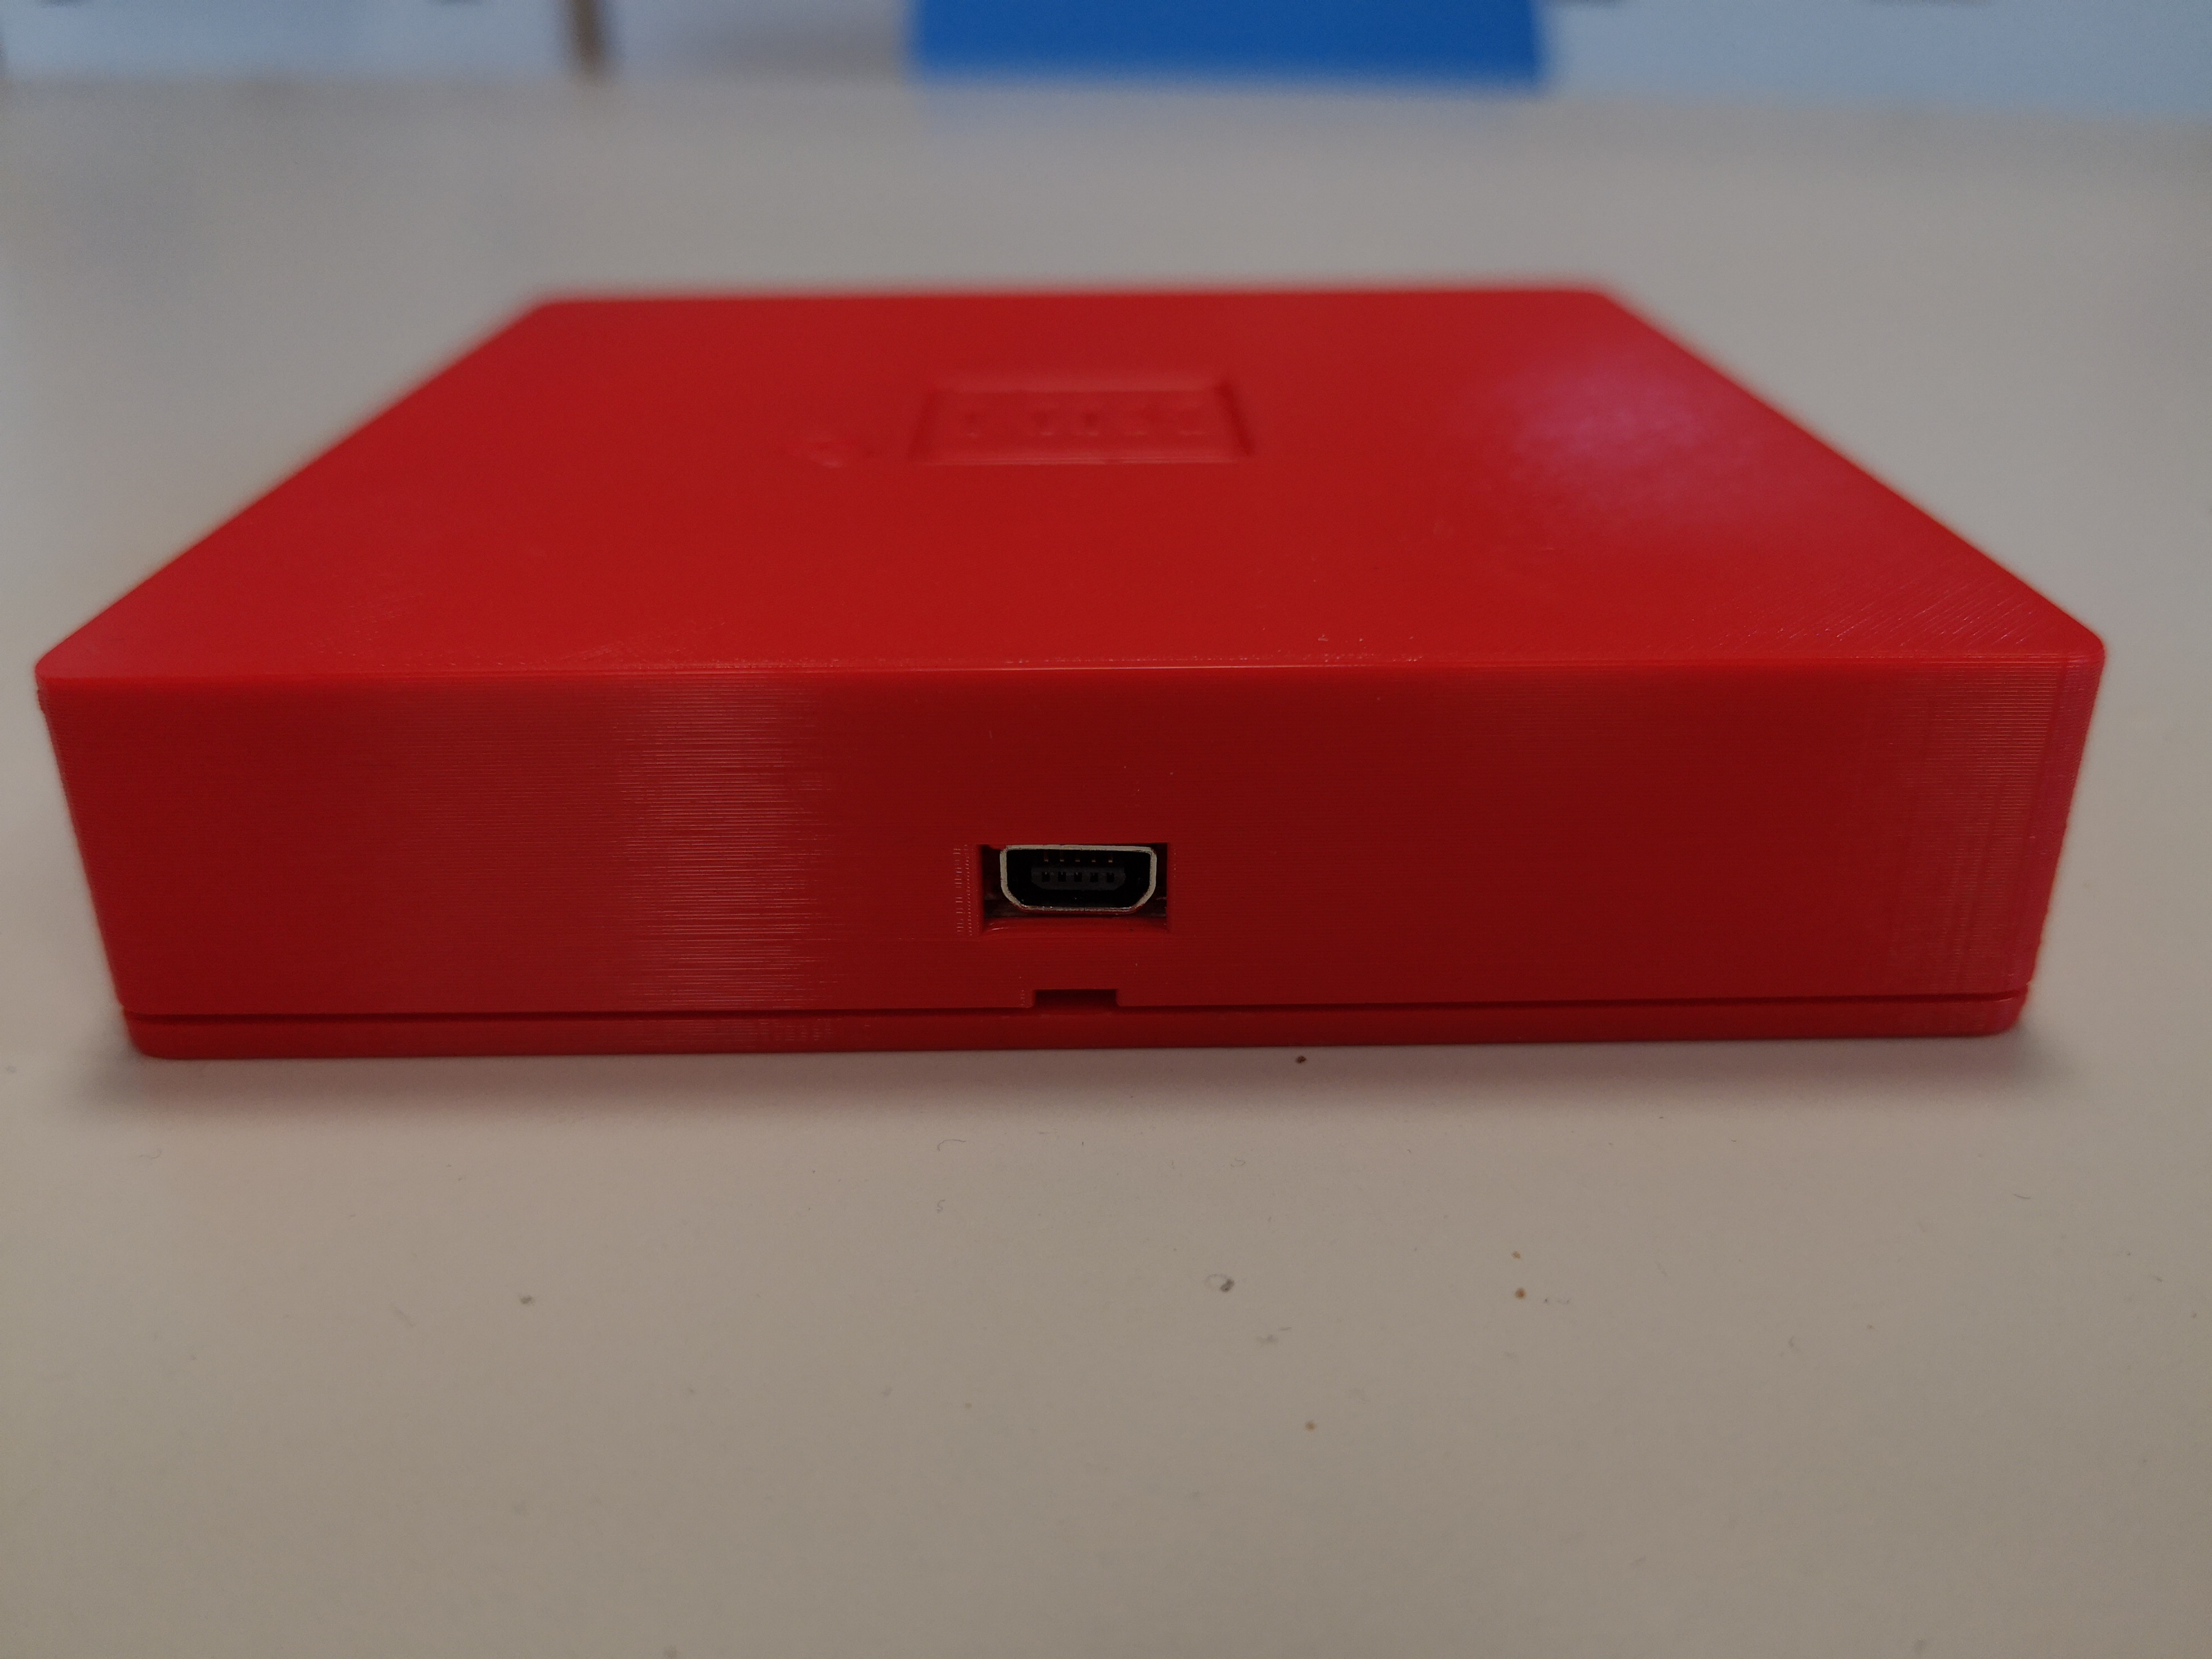
\includegraphics[width=0.4\linewidth]{../MIX_usb.jpg}
	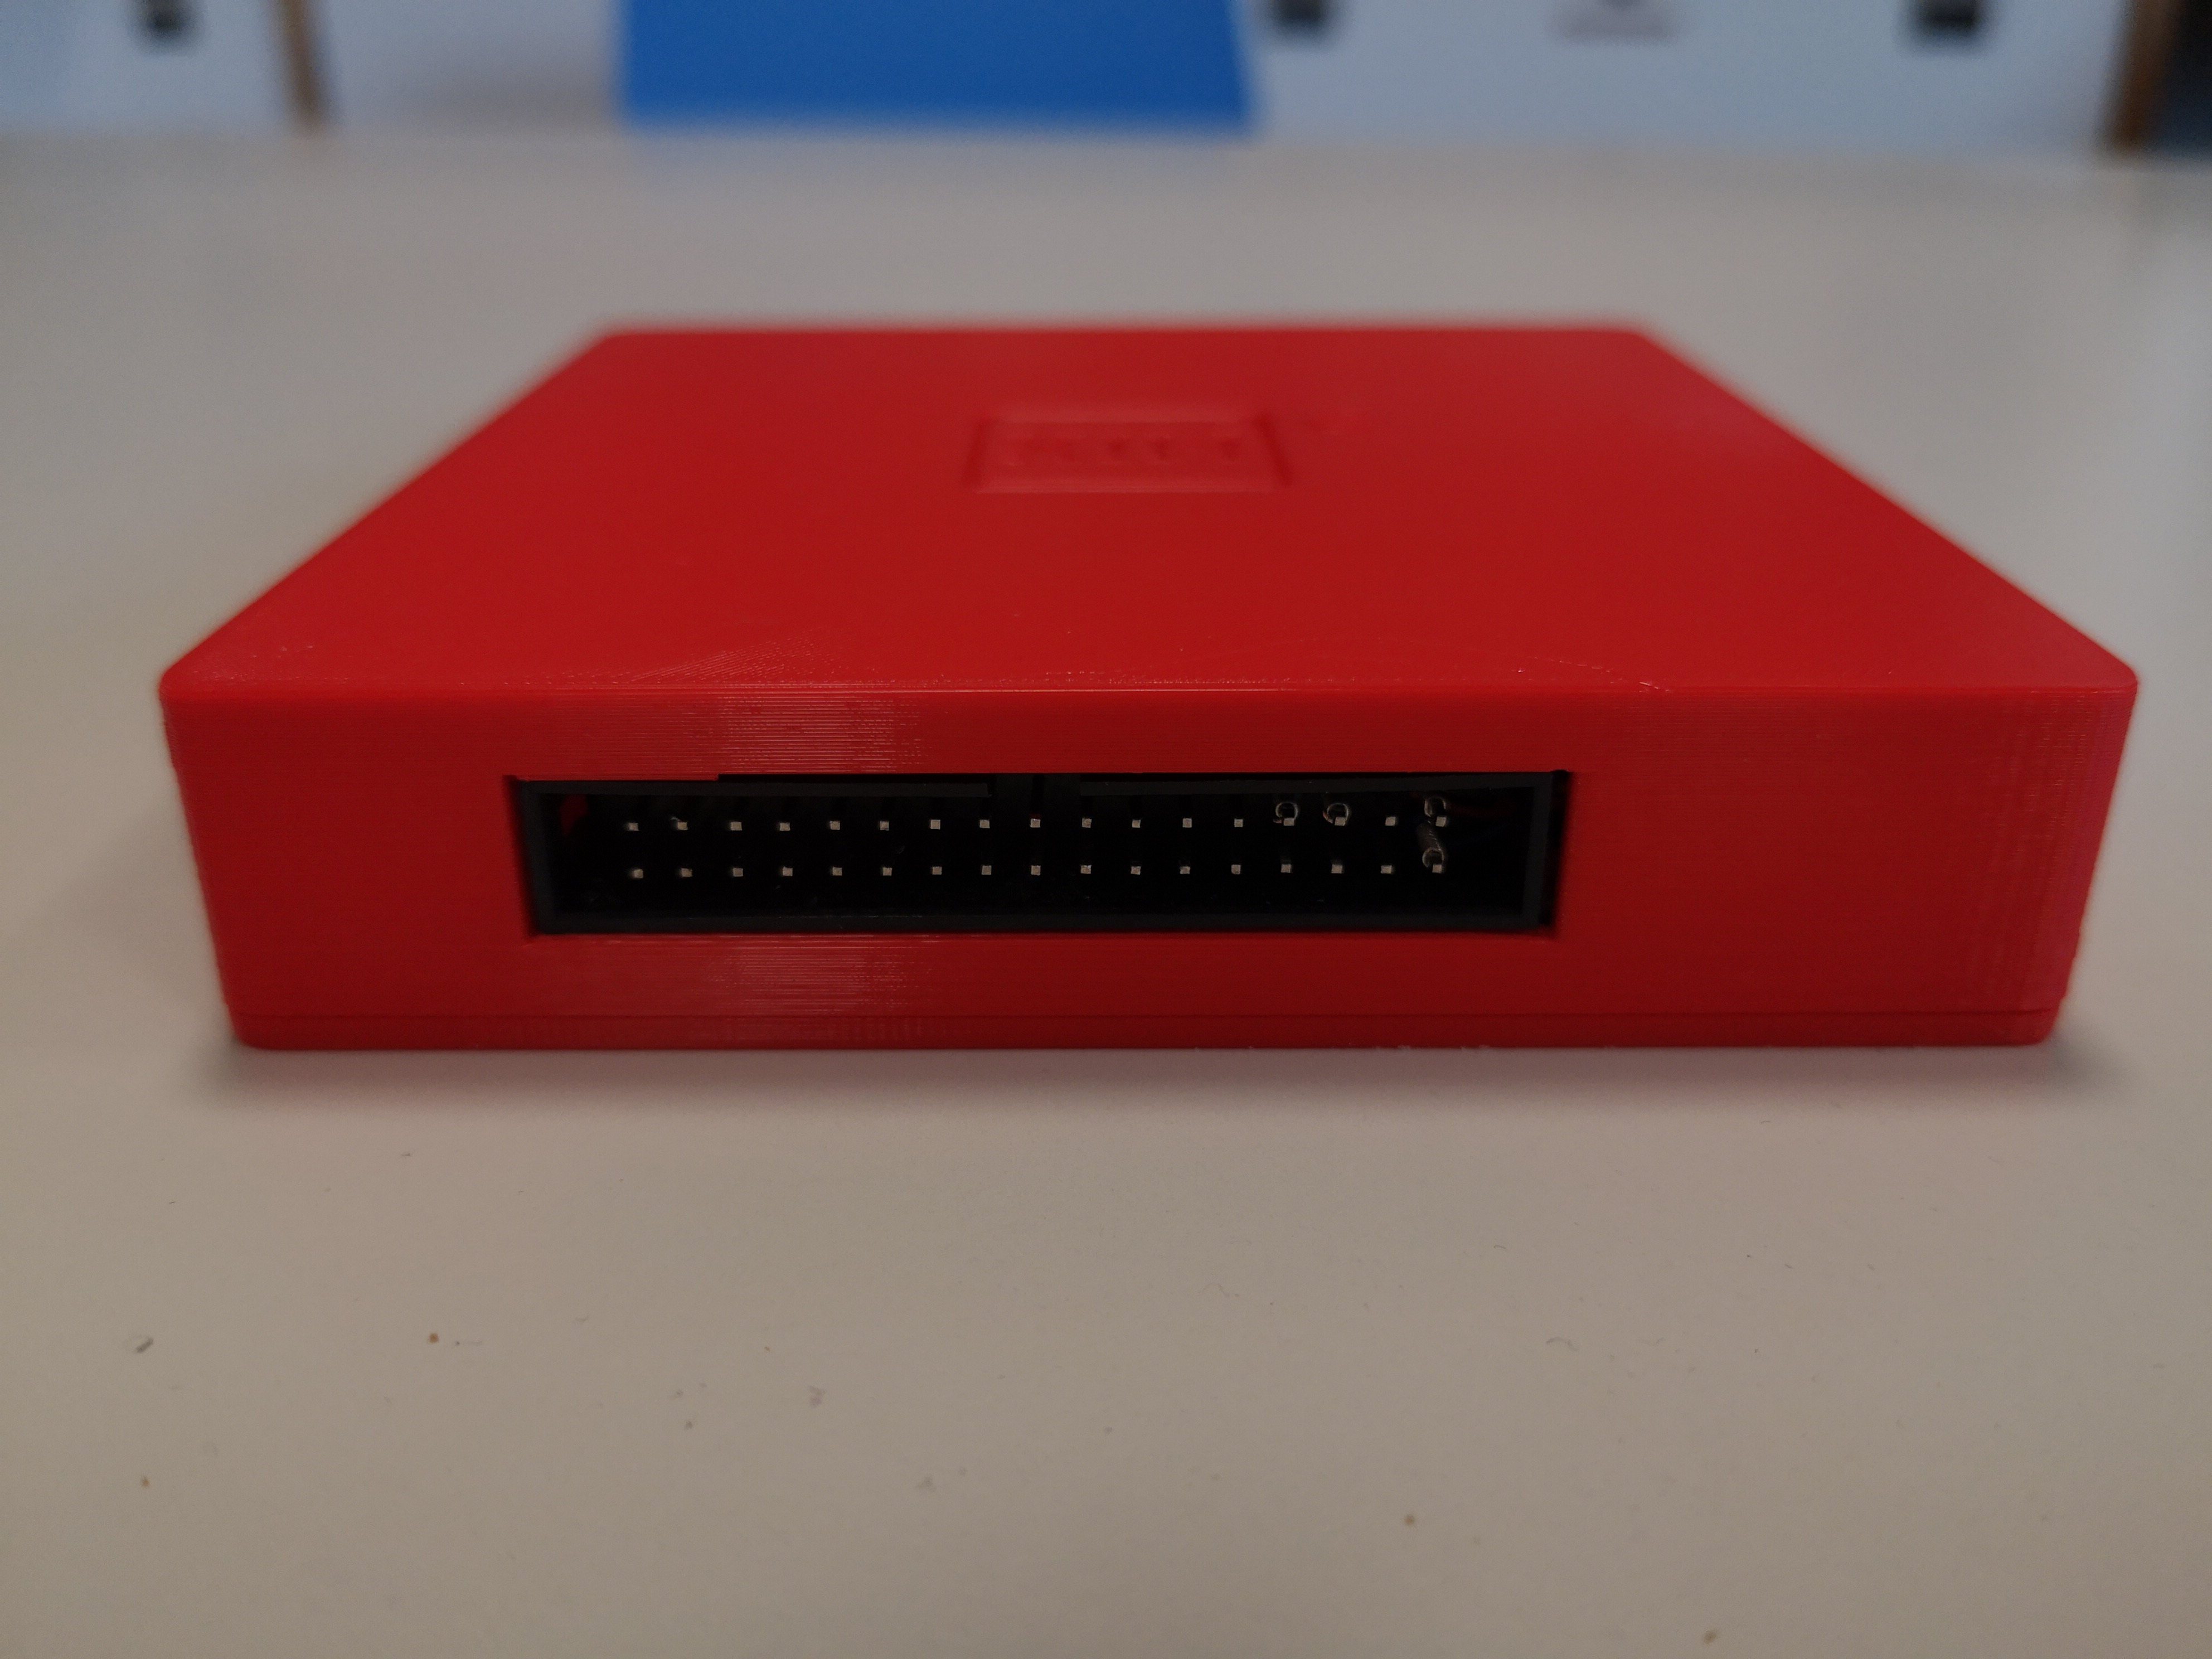
\includegraphics[width=0.4\linewidth]{../MIX_gpio.jpg}
	
	\caption{All character based I/O is done through a USB to serial adapter @115200 baud (8N1). MIX can be expanded through a GPIO connector placed at the rear side }
	\label{fig:mixusb}
\end{figure}



\subsubsection{MIX commands}
All commands exept the floating point arithmetic are implemented with execution times corresponding to Knuth's specifications. Special care is given to the correct timings. Even the \textit{sofisticated} commands \lstinline|SRC| and \lstinline|SLC|, which need a fancy modulo 10 computation are executed in the defined timing of two cycles. The system can (easily) be extended in various ways:

\begin{enumerate}
	\item more commands:
	\begin{itemize}
		\item easy: add logic operators (\lstinline|AND|, \lstinline|OR|, \lstinline|XOR|, \lstinline|NOT|)
		\item not so easy: add floating point arithmetic (\lstinline|FADD|, \lstinline|FSUB|, \lstinline|FMUL|, \lstinline|FDIV|)
		
	\end{itemize}
	\item  more hardware:
	\begin{itemize}
		\item easy: add leds to run the traffic light example (s. chapter \ref{traffic} of this manual)
		\item not so easy: add more I/O units
	\end{itemize}
	

\end{enumerate}
\subsubsection{The GO button}
MIX comes with the \textit{GO button} attached to USB-UART. So after pressing the \textit{GO button} MIX-programms can be uploaded by sending the \textit{punched cards} to USB-UART.

\subsubsection{The toast case}
MIX comes in a nice case with formfactor of a slice of toast ($\SI{10}{cm} \times \SI{10}{cm} \times \SI{2}{cm}$), so your complete MIX computer system will easily fit into your lunch box. The case can be printed with a 3D printer. Design files can be found in the directory \lstinline|build/toast| of the project site.

\section{Running programs on MIX}
\subsection{Requirement}
To run mixal programs on your MIX you need a few things:
\begin{itemize}
	\item \lstinline|mixasm|: Assembler provided in the package mdk
	\item \lstinline|python3|: Tools to translate mixal code to the various formats are written in python
	\item \lstinline|gitlab.com/x653/mix-fpga|: The authors repository of this project
	\item \lstinline|screen|: a terminal emulator to connect to MIX
\end{itemize}

Open a terminal and install the required packages:

\begin{lstlisting}[numbers=none,frame=none]
sudo apt install mdk
sudo apt install python3
sudo apt install screen
git clone https://gitlab.com/x653/mix-fpga
\end{lstlisting}

\subsection{mixasm}
To run mixal programs with MIX you first have to translate the mixal programs to machine language. This is done with the GNU tanslator \lstinline|mixasm| distributed with the mix software package  \lstinline|mdk|.

\begin{lstlisting}[numbers=none,frame=none]
mixasm <filename>.mixal -l
\end{lstlisting}

The \lstinline|-l| option is needed to create the listing file \lstinline|<filename>.mls|.


\subsection{tools}
To upload the code onto MIX we have to translate the listing in a computer readable format. For this you can use the python scripts in the subdirector \lstinline|mix-fpga/tools|:
\begin{itemize}
	\item \lstinline|mls2card.py|: translate the machine code listing (\lstinline|<filename>.mls|) to punched card format.
	\item  \lstinline|mls2char.py|: translate the listing to character codes, which can directly be read by MIX. (This is only necessary for the bootloader written on the first two punched cards).
	\item  \lstinline|mls2bin.py|: translate the listing file to binary. This is only necessary for the program \textit{go-button}, which must be uploaded directly into fpga ROM.
	 
\end{itemize}

\subsection{upload and run}
Finally you can connect your PC to MIX with a USB cable and start the  terminal emulator (\lstinline|screen|):
\begin{lstlisting}[numbers=none,frame=none]
screen /dev/ttyUSB0 115200
\end{lstlisting}
Press the \textit{go button} to start MIX. You should see the MIX welcome message:

\begin{lstlisting}
WELCOME TO MIX. 1U = 40NS. U16-U20 TO UART @115200 BAUD (8N1).        
\end{lstlisting}

If \lstinline|screen| does not open the terminal try with \lstinline|sudo screen|. This might happen, when the user is not allowed to acces the device \lstinline|/dev/ttyUSB0|. Check the user setting of \lstinline|/dev/ttyUSB0| and add the user to the linux group \lstinline|sudo usermod -a -G $USER dialout|.

Within  the screen session you can upload the mixal programs written on punch cards:
\begin{lstlisting}[language=bash,numbers=none,frame=none]
<ctr-a> : readreg p p.card
<ctrl-a> : paste p
\end{lstlisting}


\subsection{Verify}
The following programms in the folder \lstinline|mix-fpga/mixal| have been verified to run on MIX:
\begin{itemize}
	\item \lstinline|p|: compute the first 500 primes
	\item \lstinline|e|: compute easter dates from 1950 -- 2000
	\item  \lstinline|t|: control traffic signals
	\item  \lstinline|go|: the go button
	\item \lstinline|boot|: the bootloader
	\item \lstinline|coins|: calculate possible change
	\item \lstinline|perm|: calculate the product of permutations
	\item \lstinline|disk|: test the disk unit U8
\end{itemize}

\section{Example program p}
We will run programm \lstinline|p| of chapter 1.3.2 TAOCP (p. 148) on MIX. Programm \lstinline|p| computes the first 500 primes and outputs them in a table on the line printer U18.
\subsection{Prepare the input}
\subsubsection{p.mixal}
The mixal program can be found in \lstinline|mixal/p/p.mixal|:

\begin{lstlisting}[numbers=none,frame=none]
cd mixal/p
cat p.mixal
\end{lstlisting}

\lstinputlisting{../../mixal/p/p.mixal}

\subsubsection{p.mls}
First we translate the mixal programm to binary code. This is done with \lstinline|mixasm| (included in the GNU library \lstinline|mdk|). Add the option \lstinline|-l| to create the listing file \lstinline|p.mls|.

\textbf{Attention}: Notice the output at line 48: "*** Startadresse: 1000". This might differ depending on the language set in your locales. It will become important in the next step!

\begin{lstlisting}[numbers=none,frame=none]
mixasm p.mixal -l
cat p.mls
\end{lstlisting}
\lstinputlisting{../../mixal/p/p.mls}

\subsubsection{p.card}
Next we must write the binary code onto punched cards. This can be done with the python script \lstinline|mixal/tools/mls2card.py|.
The python scripts reads the listing file \lstinline|p.mls|, extracts the code and writes it in the file \lstinline|p.card|.
Every line of \lstinline|p.card| holds 80 chars of a card. The first to cards contain the bootloader discussed in exercise 26 in chapter 1.3.1 of TAOCP (see p. 510)\footnote{notice the \lstinline|J| in card 2!}. The last cards is the so called transfer card, which tells the bootloader to start execution at memory location 1000.

\textbf{Attention}: You might miss the transfer card because your output has no "*** Startadresse ...".
In this case edit the python script \lstinline|mls2card.py| and adjust to the apropriate String found in your \lstinline|*.mls| output.


\begin{lstlisting}[numbers=none,frame=none]
../../tools/mls2card.py p.mls
cat p.card
\end{lstlisting}

\lstinputlisting{../../mixal/p/p.card}


\subsection{How to send the cards to MIX}
\subsubsection{go button}
Power MIX with USB cable connected to your computer.
Start a screen session with 115200 baud (8N1)
\begin{lstlisting}[numbers=none,frame=none]
screen /dev/ttyUSB0 115200
\end{lstlisting}

Press the \textit{Go button} on MIX. You should see the welcome message on your terminal:
\begin{lstlisting}
WELCOME TO MIX. 1U = 40NS. U19 @115200 BAUD (8N1).                    
\end{lstlisting}

\subsubsection{input the cards to U16}
You can now send the punched cards to MIX within the screen terminal session.
Read cards into a screen-buffer (called p) and send the buffer to MIX.
\begin{lstlisting}[numbers=none,frame=none]
<in screen terminal> Ctr-a : readreg p p.card <enter>
<in screen terminal> Ctrl-a : paste p <enter>
\end{lstlisting}

After a short amount of time MIX spits out the following table to the printer U18. Notice that output to U18 have 120 characters per line, while output to the terminal U19 is only 70 chars wide.
\lstinputlisting{../../mixal/p/p.out}

\subsection{Congratulation}
You have run your first program on a \textit{real} MIX.
Now trun the program \lstinline|e| to calculate the easter dates.

\section{Build your own MIX and/or modify the fpga design}

In this section we will show how to build a MIX based on the fpga board iCE40HX8K-EVB. The whole project uses only FOSS soft- and hardware. With little modifications it should run on any fpga board available out in the wild.

\subsection{Requirement}
\begin{enumerate}
	\item 
	fpga board (iCE40HX8K-EVB)
	\item programmer device (Olimexino 32u4) with idc10 cable (cable-IDC10)
	\item USB-UART-board (BB-CH340T).  
	\item fpga toolchain. The project was developed with \lstinline|apio| \footnote{\href{github.com/FPGAwars/apio}{github.com/FPGAwars/apio}}, a software suite based on project icestorm\footnote{\href{www.clifford.at/icestorm}{www.clifford.at/icestorm}} from Clifford Wolf.
\end{enumerate}

Consider to buy at Olimex Ltd. \footnote{\href{www.olimex.com}{www.olimex.com}}, the company with the highest number of registered OSHW-projects. Install the tools with:

\begin{lstlisting}[numbers=none,frame=none]
sudo pip install -U apio
apio install -ice40
apio install -iverilog
apio install -scons
apio install -yosys
sudo apt install gtkwave
cd tools/iceprogduino
make
sudo make install
\end{lstlisting}

\subsection{build and flash the fpga design}

Cd into the directory \lstinline|build/rtl| and build the project. Connect the fpga board with olimexino-32u4 programmer to upload the bitstream file. Use two USB cables to power both boards.

\begin{figure}[H]
	\centering
	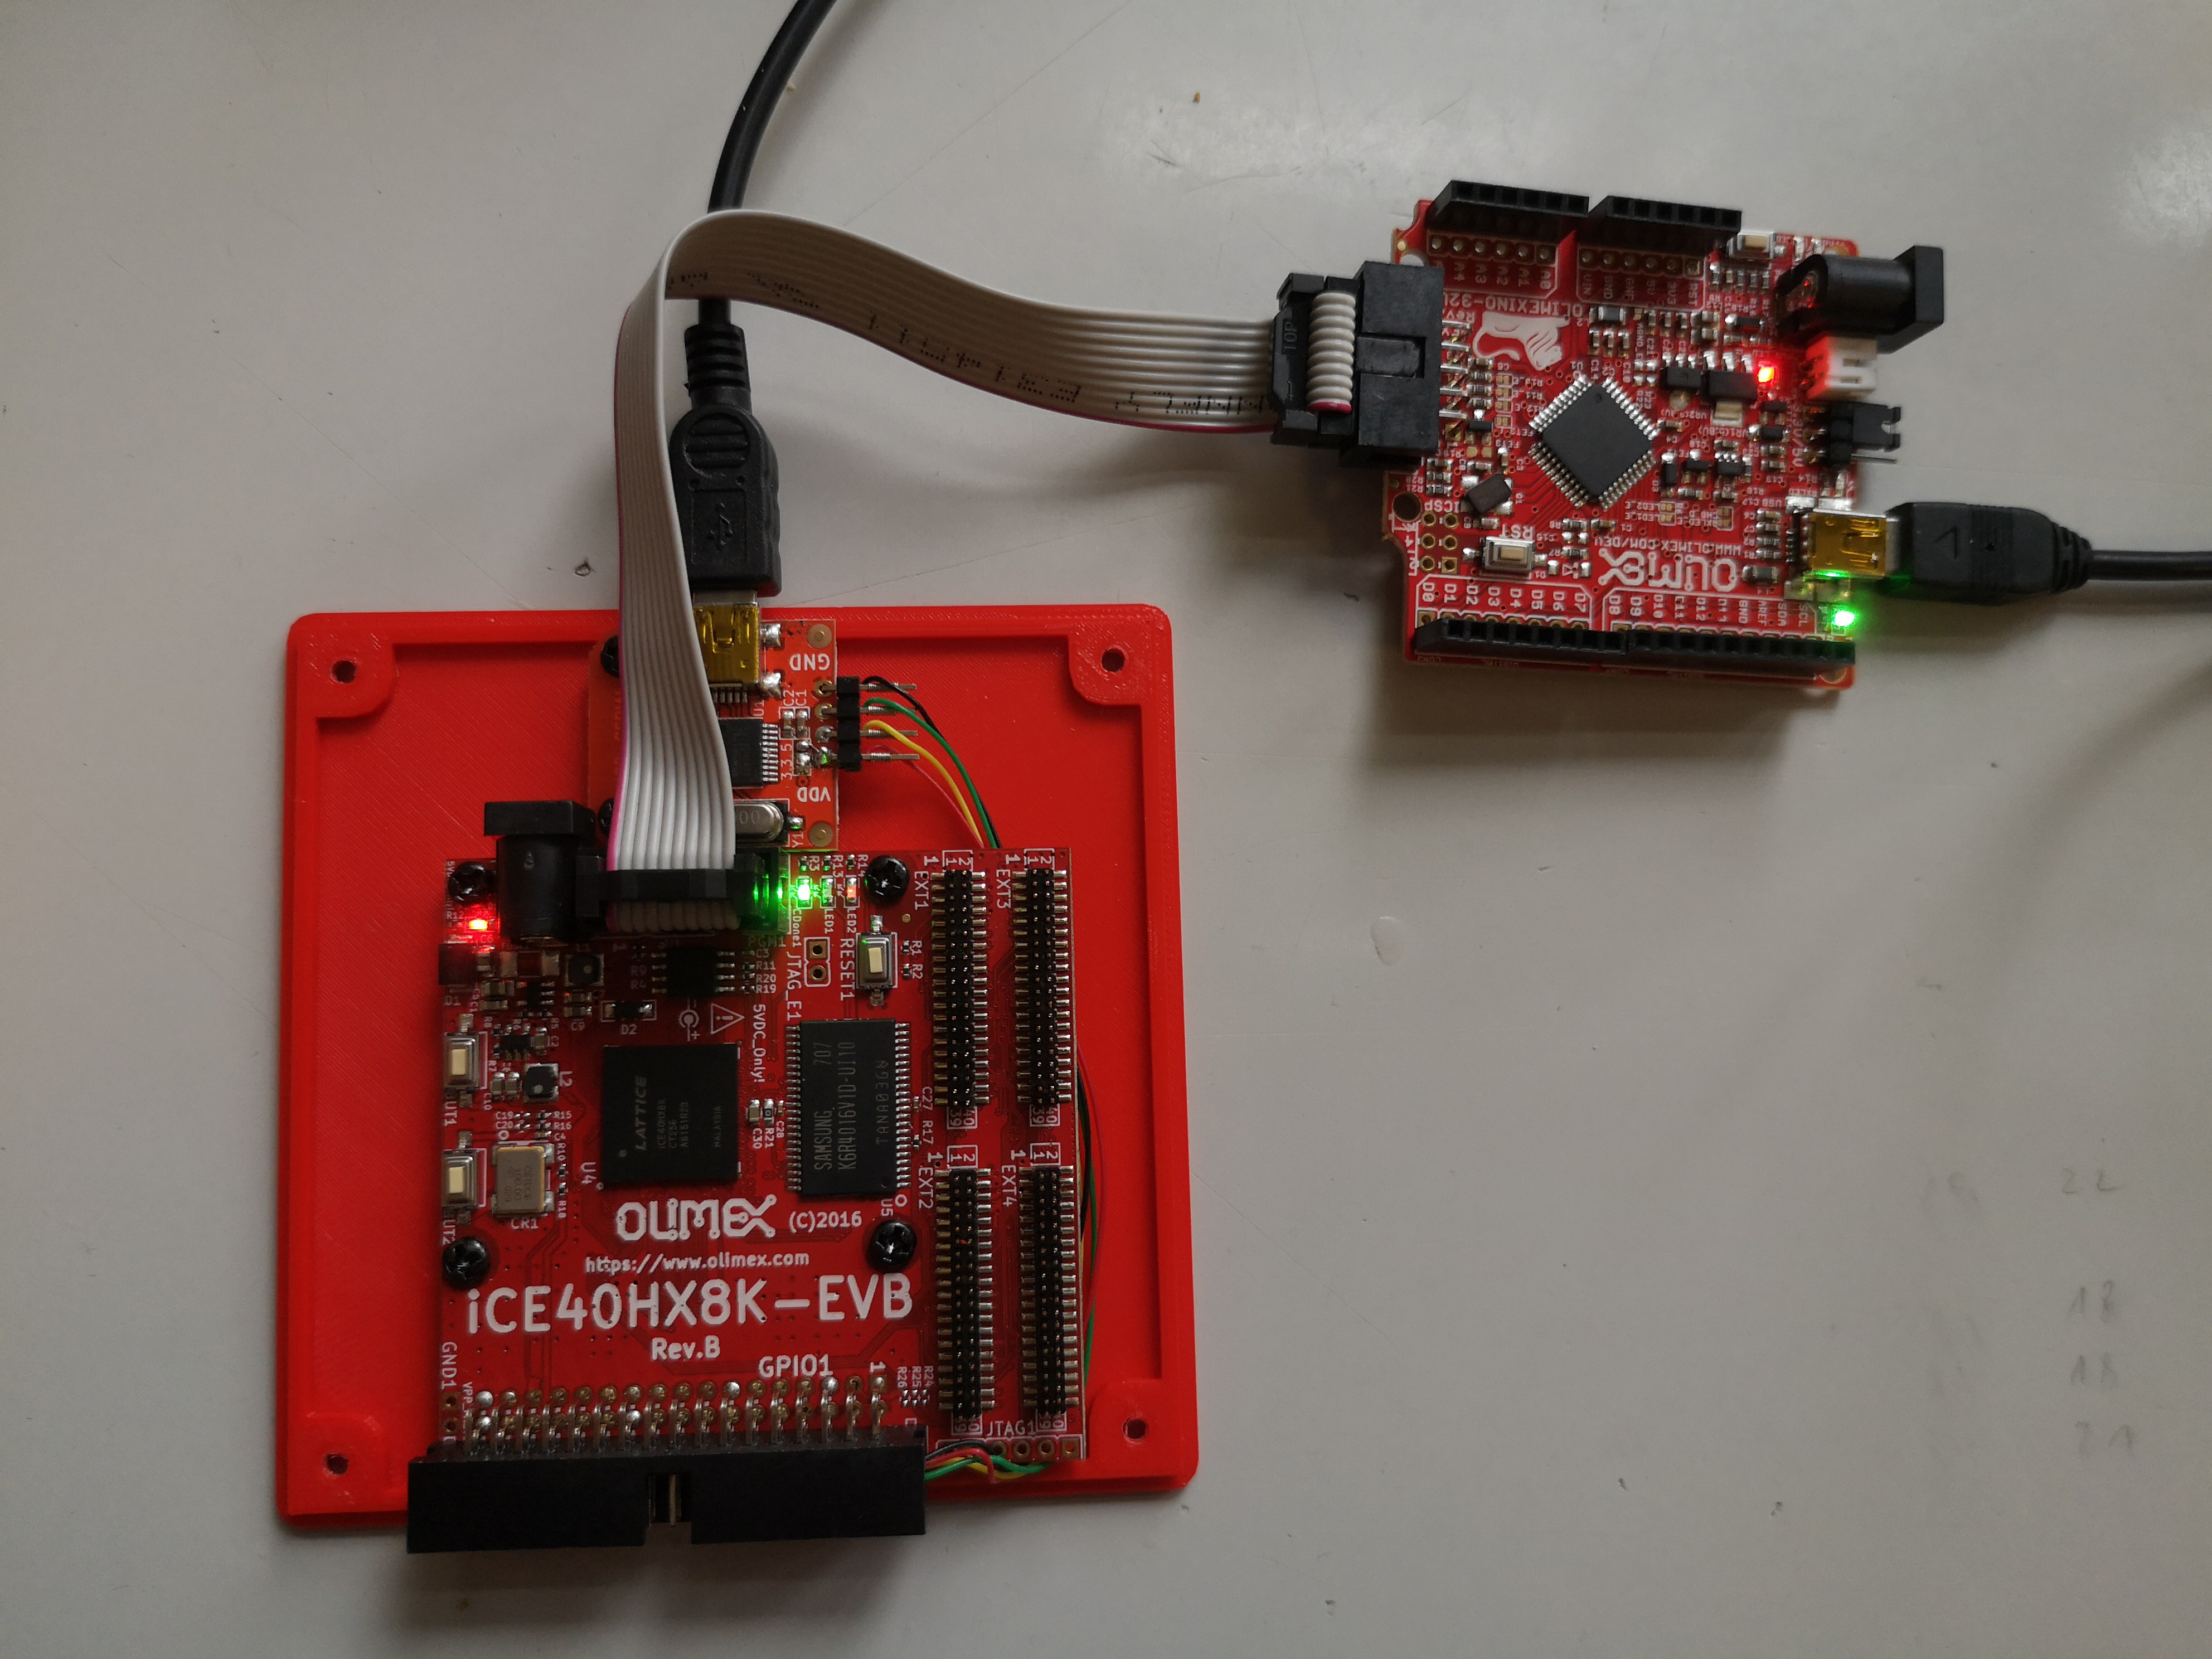
\includegraphics[width=0.6\linewidth]{../MIX_flash.jpg}
	\caption{Connect programmer Olimexino-32u4 with fpga board iCE40HX8K-EVB}
	\label{fig:flash}
\end{figure}


\begin{lstlisting}[numbers=none,frame=none]
cd build/rtl
apio clean
apio build -v
apio upload
\end{lstlisting}

\subsection{The USB-serial adapter}
To connect the USB-UART-board (BB-CH340T) with iCE40HX8K-EVB we first have to modify BB-CH340T according to Fig. \ref{fig:detail}: To use USB-Serial adapter as power source we must cut with a cutter knife the pcb track marked in GREEN and solder a bridge BLACK between the right most terminal (VDD) and the 5V pad.
This will ensure that the right most terminal connector (red cable) get's 5Volt, which will be used to power the fpga board. But the UART signals (green and yellow cables) are still leveled to 3.3V, which corresponds to the in-/output signal level of fpga-connector GPIO1.
\begin{figure}[H]
	\centering
	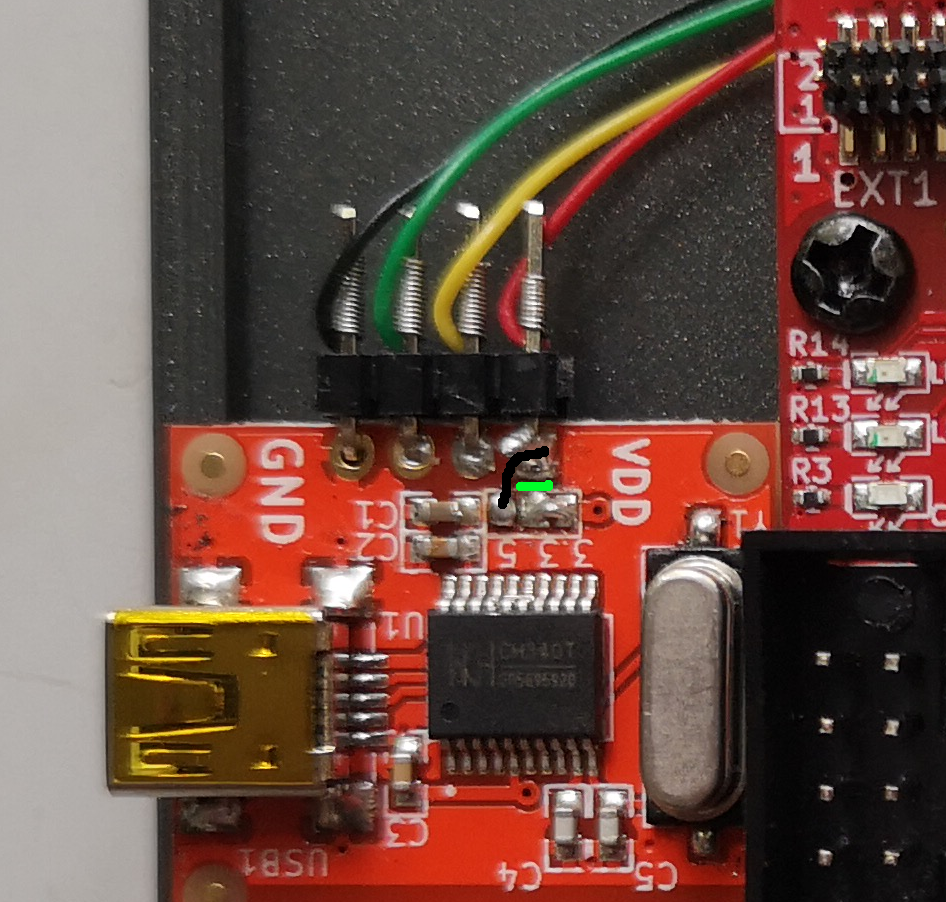
\includegraphics[width=0.6\linewidth]{../detail.png}
	\caption{Cut the pcb track (GREEN) and solder a bridge from 5V pad to the right most connector pin.}
	\label{fig:detail}
\end{figure}

The 4 wires are connected to the GPIO connector on the right side of iCE40HX8K-EVB according to the following table. Compare with schematic in the appendix  \ref{sec:schematic}.

\begin{table}[H]
	\centering
	
	\begin{tabular}{|c|c|c|}
		\hline 
		color & USB-serial & GPIO (ICE40HX8K-EVB) \\ 
		\hline 
		black & GND & 2 \\ 
		\hline 
		green & RX & 7 \\ 
		\hline 
		yellow & TX & 5 \\ 
		\hline 
		red & VDD & 1 \\ 
		\hline 
	\end{tabular} 
\end{table}


\subsection{The Go button}
We will implement the code needed by the go button proposed in  exercise 26 in chapter 1.3.1 of TAOCP (see p. 510).

\subsubsection{prepare the software}
The mixal program can be found in \lstinline|go.mixal|. It starts at location 4000 (which is implemented in fpga but not used by MIX). The programm spits out the welcome message. The JMP instruction at memory cell 4095 will jmp to location 0 storing a +0000 in the J-Register, because beeing a binary version with 12 bit programmcounter the next execution address without the jmp instruction would equally yield 4095 + 1 = 0000.


\lstinputlisting{../../mixal/go/go.mixal}

First we compile the mixal programm to binary code with \lstinline|mixasm|. Then we translate the listing file to a binary representation, which can be directly written to the fpga board.

\begin{lstlisting}[numbers=none,frame=none]
mixasm go.mixal -l
../../tools/mls2bin.py go.mls
cat go.bin
\end{lstlisting}

The python scripts reads the listing file \lstinline|go.mls|, extracts the code and writes it in the file \lstinline|go.bin|.

\begin{lstlisting}
0000000000000000000000000000000
0000000000000000000000000000000
0000000000000000000000000000000
...
...
0000000000000000000000000000000
0111110100001000000010011100101
0111111111100000000010011100010
0000000000000000000010000100100
0111111111110000000010000100010
0000000000000000000000000100111
\end{lstlisting}

The output contain the program code expressed as binary numbers. These binary numbers can be flashed to the iCE40HX8K-EVB board, so it will be stored permanently in the MIX computer. At every reset (press \textit{Go button}) the code will be executed. The first 4000 zero lines translate to NOP instructions. At the end you find the sequence IN(16),JBUS,JMP...

\subsection{rebuild and flash to iCE40HX8K-EVB}

\begin{itemize}
	\item Copy the binary file \lstinline|go.bin| into the directory \lstinline|rtl|, where the fpga description files are.
	\item Rebuild the fpga project and upload. An \lstinline|apio clean| is needed, because otherwise the preloaded memory will not be updated.	
\end{itemize}

\begin{lstlisting}[numbers=none,frame=none]
cp go.bin ../../rtl/go.bin
apio clean
apio build -v
apio upload
\end{lstlisting}

\textbf{Tipp:} change the welcome message to ensure the new rom file has been uploaded.

\section{Example program t}
\label{traffic}
We will run programm \lstinline|t| of exercise 20 in chapter 1.3.2 TAOCP (p. 161) on MIX. Programm t controls the traffic signal at corner of Del Mare Boulevard and Berkeley Avenue. This project will connect LEDs directly to the register rX and a push button to the  Overflow toggle. This will be done extending the fpga design and routing the appropriate signals to the GPIO connector at the back of MIX.

\begin{figure}[H]
	\centering
	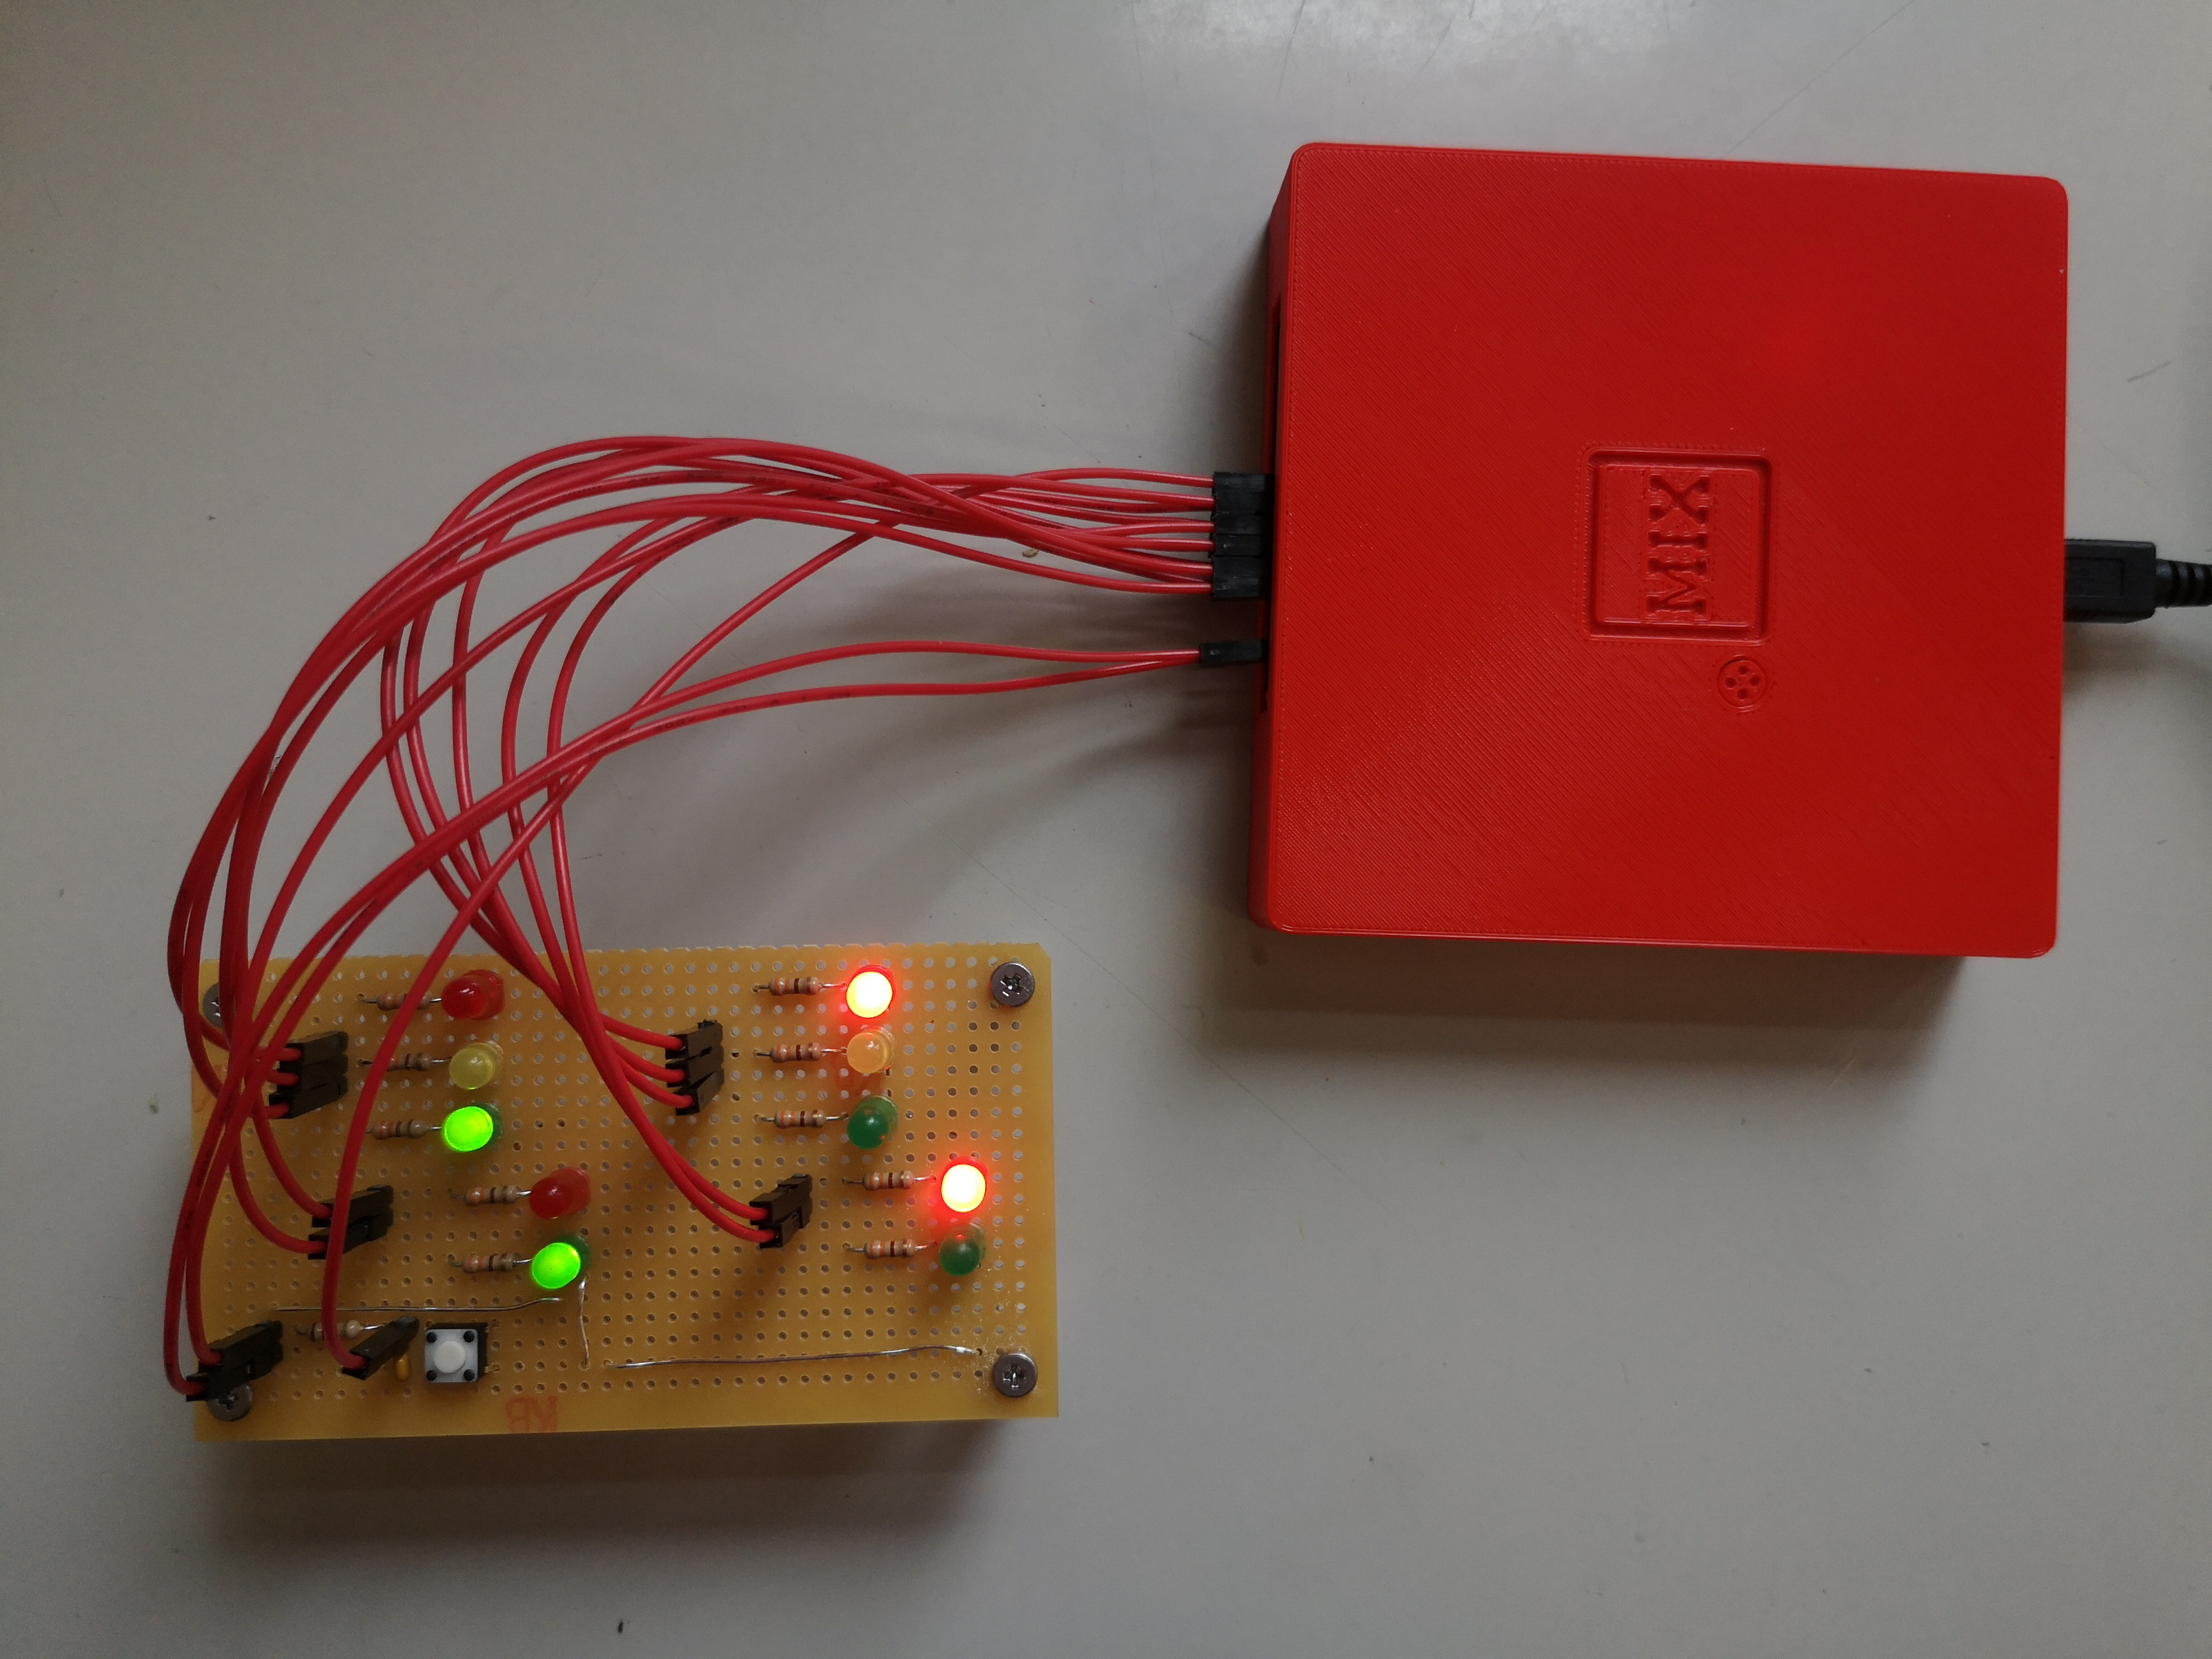
\includegraphics[width=0.7\linewidth]{../MIX_traffic}
	\caption{Connect LEDs and push button over the GPIO connector directly to register rX to control the traffic light}
	\label{fig:mixtraffic}
\end{figure}


\subsection{Extending the fpga desing}

Make a copy of the folder \lstinline|rtl| and cd into it.

\begin{lstlisting}[numbers=none,frame=none]
cd build
cp -r rtl rtl_traffic_light
cd rtl_traffic_light
\end{lstlisting}


\subsubsection{mix.pcf}

Find the following lines in the physical constraint file \lstinline|mix.pcf| and uncomment.

\lstinputlisting{mix.pcf}

\subsubsection{mix.v}

To connect the Register rX with the traffic signals: find the following lines in \lstinline|mix.v| and uncomment:

\lstinputlisting{mix1.v}

Control the overflow toggle with the button by uncommenting line 7 in the code snippet:

\lstinputlisting{mix2.v}

\subsection{rebuild and flash to iCE40HX8K-EVB}

Rebuild the fpga project and upload.

\begin{lstlisting}[numbers=none,frame=none]
apio clean
apio upload -v
\end{lstlisting}

\textbf{Tipp}: change the welcome message to ensure the new rom file has been uploaded.

\subsection{add leds and button to GPIO}
Connect leds and button (don't forget resistors) to the appropriate GPIO connectors as described in the \lstinline|mix.pcf| file. For simplicity only one LED is shown below:

\begin{figure}[H]
	\centering
	\input{schaltung_gpio_led.cir}

\end{figure}


\textbf{Attention}: gpio pins 1,2,5 and 7 are already used by the internal USB-serial converter.


\subsection{t.mixal}
Compile and write \lstinline|t.mixal| to puching card format. Start MIX by pressing the \textit{go button}. Upload \lstinline|t.card| to MIX and see the traffic signals blinking.


\section{Service}
In case you encounter an issue with MIX:
\begin{itemize}
	\item don't panic
	\item plese send an email to the author with a precise description of the problem.
\end{itemize}

\section{License}

\subsection{mix-fpga}
The project as a whole is licensed under the GPL 3 and can be found at \href{www.gitlab.com/x653/mix-fpga}{www.gitlab.com/x653/mix-fpga}.
\subsection{Manual}
\doclicenseThis

\newpage

\appendix

\section{Schematic iCE40HX8K-EVB}
\label{sec:schematic}
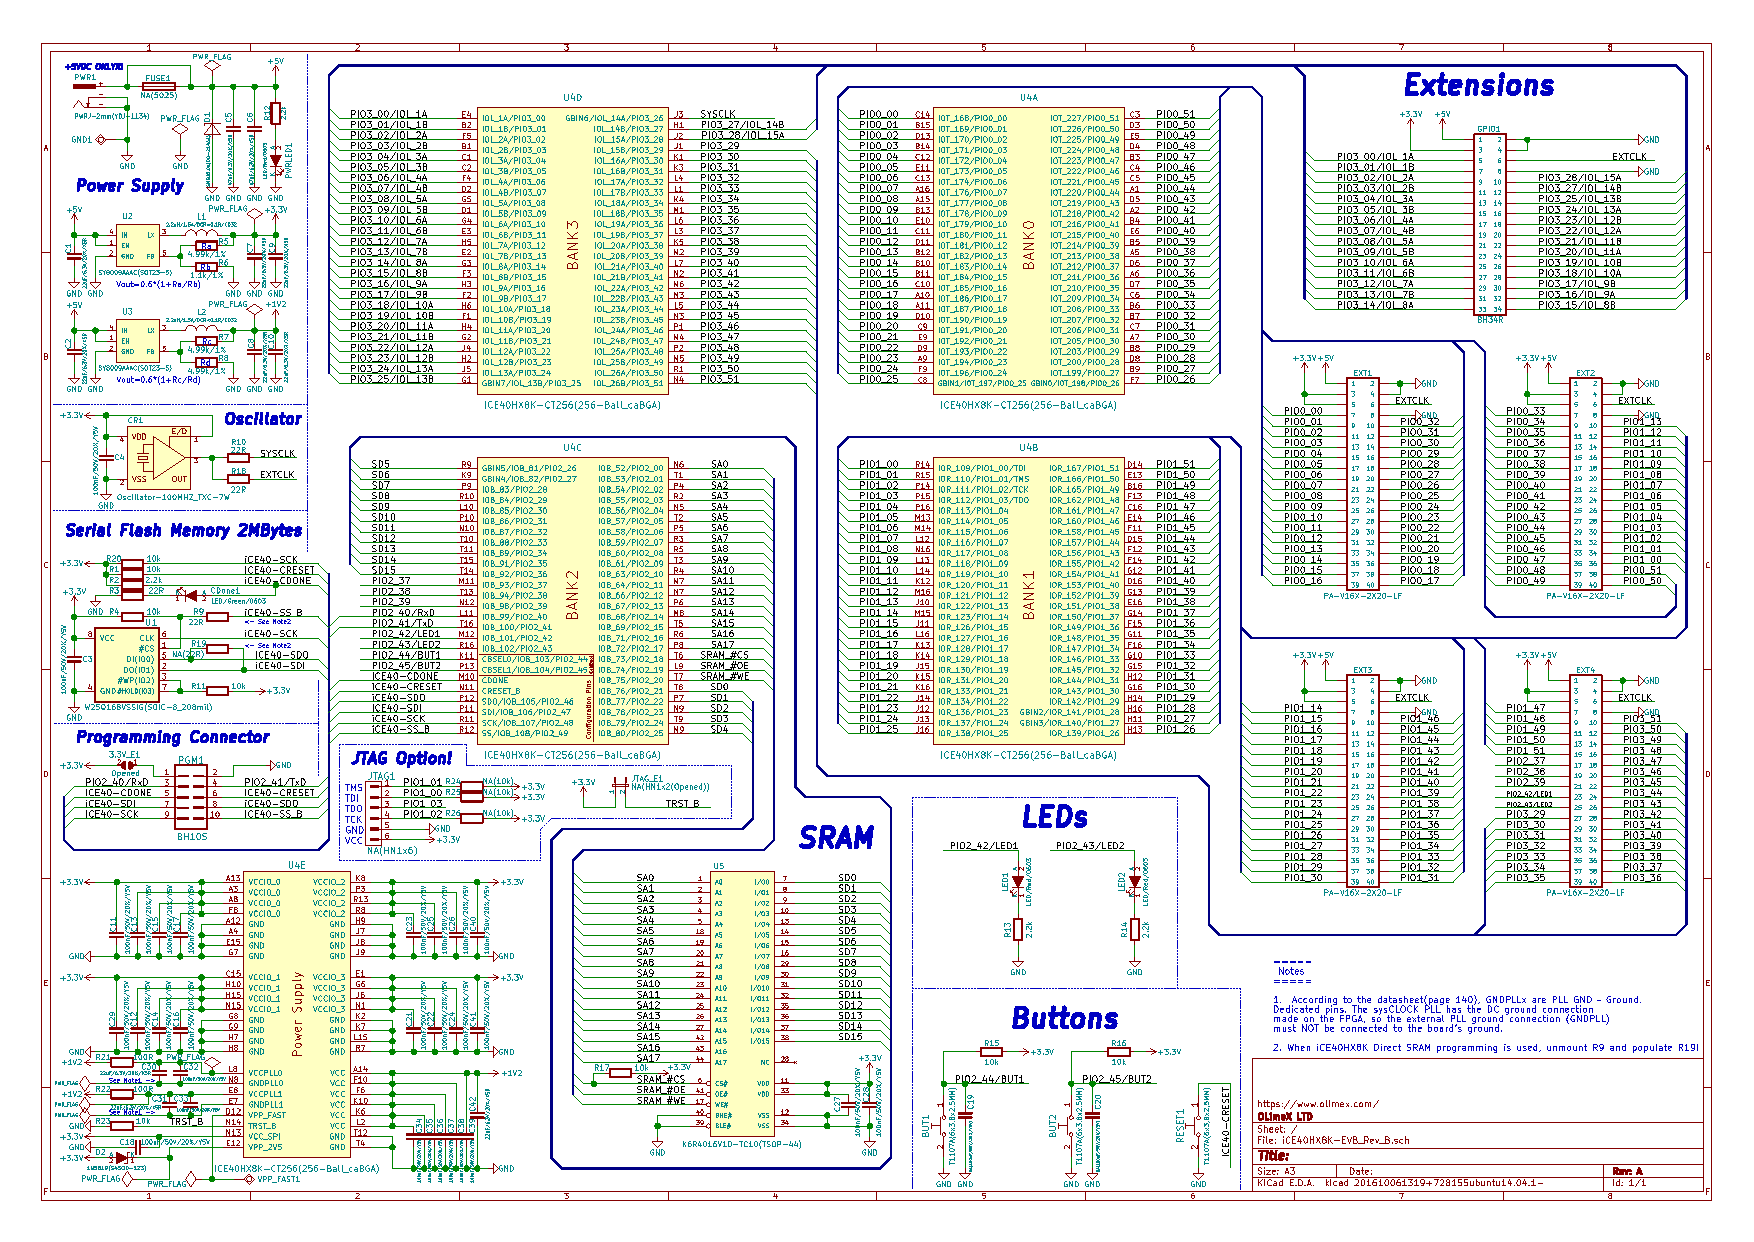
\includegraphics[angle=90,scale=0.8]{../iCE40HX8K-EVB.pdf}


\end{document}
